%*******10********20********30********40********50********60********70********80
\chap{Background Theory}
    
\section{Agile Software Development} \label{Agile}

Agile is a philosophy in software development, based on the idea of "iteration". That is, working incrementally, instead of doing everything at once. Each iteration consists on:
\begin{itemize}
\setlength{\itemsep}{-5pt}
\item Plan: What do the app have to do?
\item Design: How we want to it to behave and show?
\item Build: Code it
\item Test: Try it
\item Review: Is there something which does not work properly?
\end{itemize}

\begin{figure}[H]
	\centering
    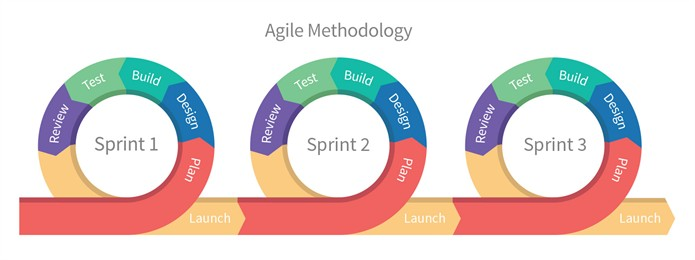
\includegraphics[trim={0 0 0 0},clip,width=0.5\textwidth]{Files/agile.jpg}
    \caption{Agile diagram.\\ \textbf{Source:}https://www.linkedin.com/pulse/agile-lean-ux-anthony-miller}
    \label{fig: Agile}
\end{figure}
The \textit{Plan} will be done by \textbf{User Stories}. A user story is a very simple way to write a thing which the software (the application, in this case), has to do. This story has to include the smallest problem possible. That is, is a problem can be divided into smaller problems, each of these lasts will be a story by itself. In order to write a correct user story, it has to answer to the following statement:
\begin{center}
\textit{As a (role) I want (something) so that (benefit).}
\end{center}
For example: \textit{As a public user, I want to create a new account so that I will have got a profile}\\
A story also will have a priority (i.e. should, mandatory) and a estimated workload: in this project, a Fibonacci sequence from 1 to 13 has been used for this purpose (the easier story will de labelled with 1 and the most difficult, with 13). There are so many ways of doing user stories; this group have been using the web platform \href{https://www.pivotaltracker.com/}{Pivotal Tracker}.
\cite{agile:modeling} 
\cite{agile:nutshell}
\section{Ruby on Rails} 
Ruby on Rails, or simply Rails, is a server-side web application framework written in Ruby under the MIT License. Rails is a model–view–controller (MVC) framework, providing default structures for a database, a web service, and web pages. \cite{wiki:RoR}

\begin{figure}[H]
	\centering
    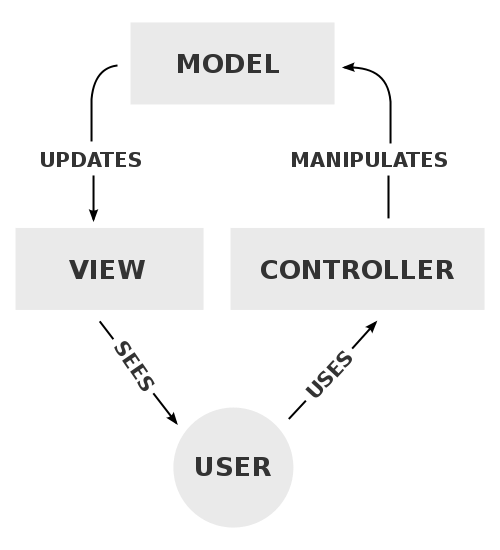
\includegraphics[trim={0 0 0 0},clip,width=0.5\textwidth]{Files/MVC.png}
    \caption{Diagram of interactions within the MVC pattern.\\ \textbf{Source:} https://en.wikipedia.org/wiki/Model-view-controller}
    \label{fig: MVC}
\end{figure}




\textbf{The Model:}
\vspace{-5mm}
\begin{itemize}
 \setlength{\itemsep}{-5pt}
\item Contains data for the application (often linked to a database)
\item Contains state of the application (e.g. what orders a customer has)
\item  Contains all business logic
\item Notifies the View of state changes (** not true of ROR, see below)
\item No knowledge of user interfaces, so it can be reused
\end{itemize}

\textbf{The View:}
\vspace{-5mm}
\begin{itemize}
 \setlength{\itemsep}{-5pt}
\item Generates the user interface which presents data to the user
\item Passive, i.e. doesn’t do any processing
\item Views work is done once the data is displayed to the user.
\item Many views can access the same model for different reasons
\end{itemize}

\textbf{The Controller:}
\vspace{-5mm}
\begin{itemize}
 \setlength{\itemsep}{-5pt}
\item Receive events from the outside world (usually through views)
\item Interact with the model
\item Displays the appropriate view to the user
\end{itemize}

https://stackoverflow.com/questions/1931335/what-is-mvc-in-ruby-on-rails




